\section{Data understanding} \label{seq:data_understanding}

 In this step the objective is to consider the available data, understand their properties, check its quality and explore it through statistical methods.

 \subsection{Collect initial data}

The data is collected through a platform called \textit{ballchasing.com} that allows players to download a plugin for the game that will automatically load their replays to to platform.

The replays are then viewable into a web based frontend and is possible to analyze different statistics from the replay. The platform provides also different HTTP API:

\begin{itemize}
    \item Get replay: returns the binary replay file given the ID;
    \item Get replay list: returns a json involving summary of replays (including the ID to get the full replay) given different filters;
    \item Get replay statistics: returns a full detailed statistics of the game for each player given the replay ID;
    \item Upload replay: used by the plugin to upload replays;
    \item Delete replay.
\end{itemize}

It is important to clarify that a replay is not a video file as usual, but a large binary file containing various metadata on the match and the players and a table in which are listed all the information necessary to review the match.
Therefore, for each instant \textit{(frame)} of the game, are listed position, direction and velocity vector of each player and the ball, and also other information of the input the players (e.g. player is using boost, player is drifting, etc...).

Extracting features from the raw replays can be very challenging, and the amount of possible features is quite high. However, the main problem about raw replays is API limitations, as it is possible to download only 200 replays per hour. Instead, we can download the replay statistics, as they are very detailed and provide stats about all the players, furthermore the limitation is 2000 per hour.

Thus, in this project, we used the calculated stats from the APIs. Each downloaded replay is saved in a JSON file. These, are hierarchical files contain also a lot of metadata and other useless for our task information about the match (e.g. stadium, car personalization of each player etc...). We discarded this data and take the stats about the six players in the match, which then results in 6 rows for each replay.

Data was collected using \textit{random sampling} from the date. The date is sampled from a range starting from August 2021 until February 2022, that's because are the dates of the two last \textit{"Seasons"} of Rocket League. At the end of each season there is a soft reset of ranks: the MMR doesn't change but the players have to do again 10 matches where the MMR change at the end of the match is higher.
I decided to not consider older seasons because the \textit{playstyle} and the distribution of players in Rocket League changes over time.

However, we have to discard some player rows where the rank information was missing. This is due to the fact that the rank in that match wasn't determined yet.

\subsection{Describe data}

The resulting dataset counts \note{data len} rows. Let's examine the dataset statistics:

\begin{figure}[H]
    \resizebox{1.1\linewidth}{!}{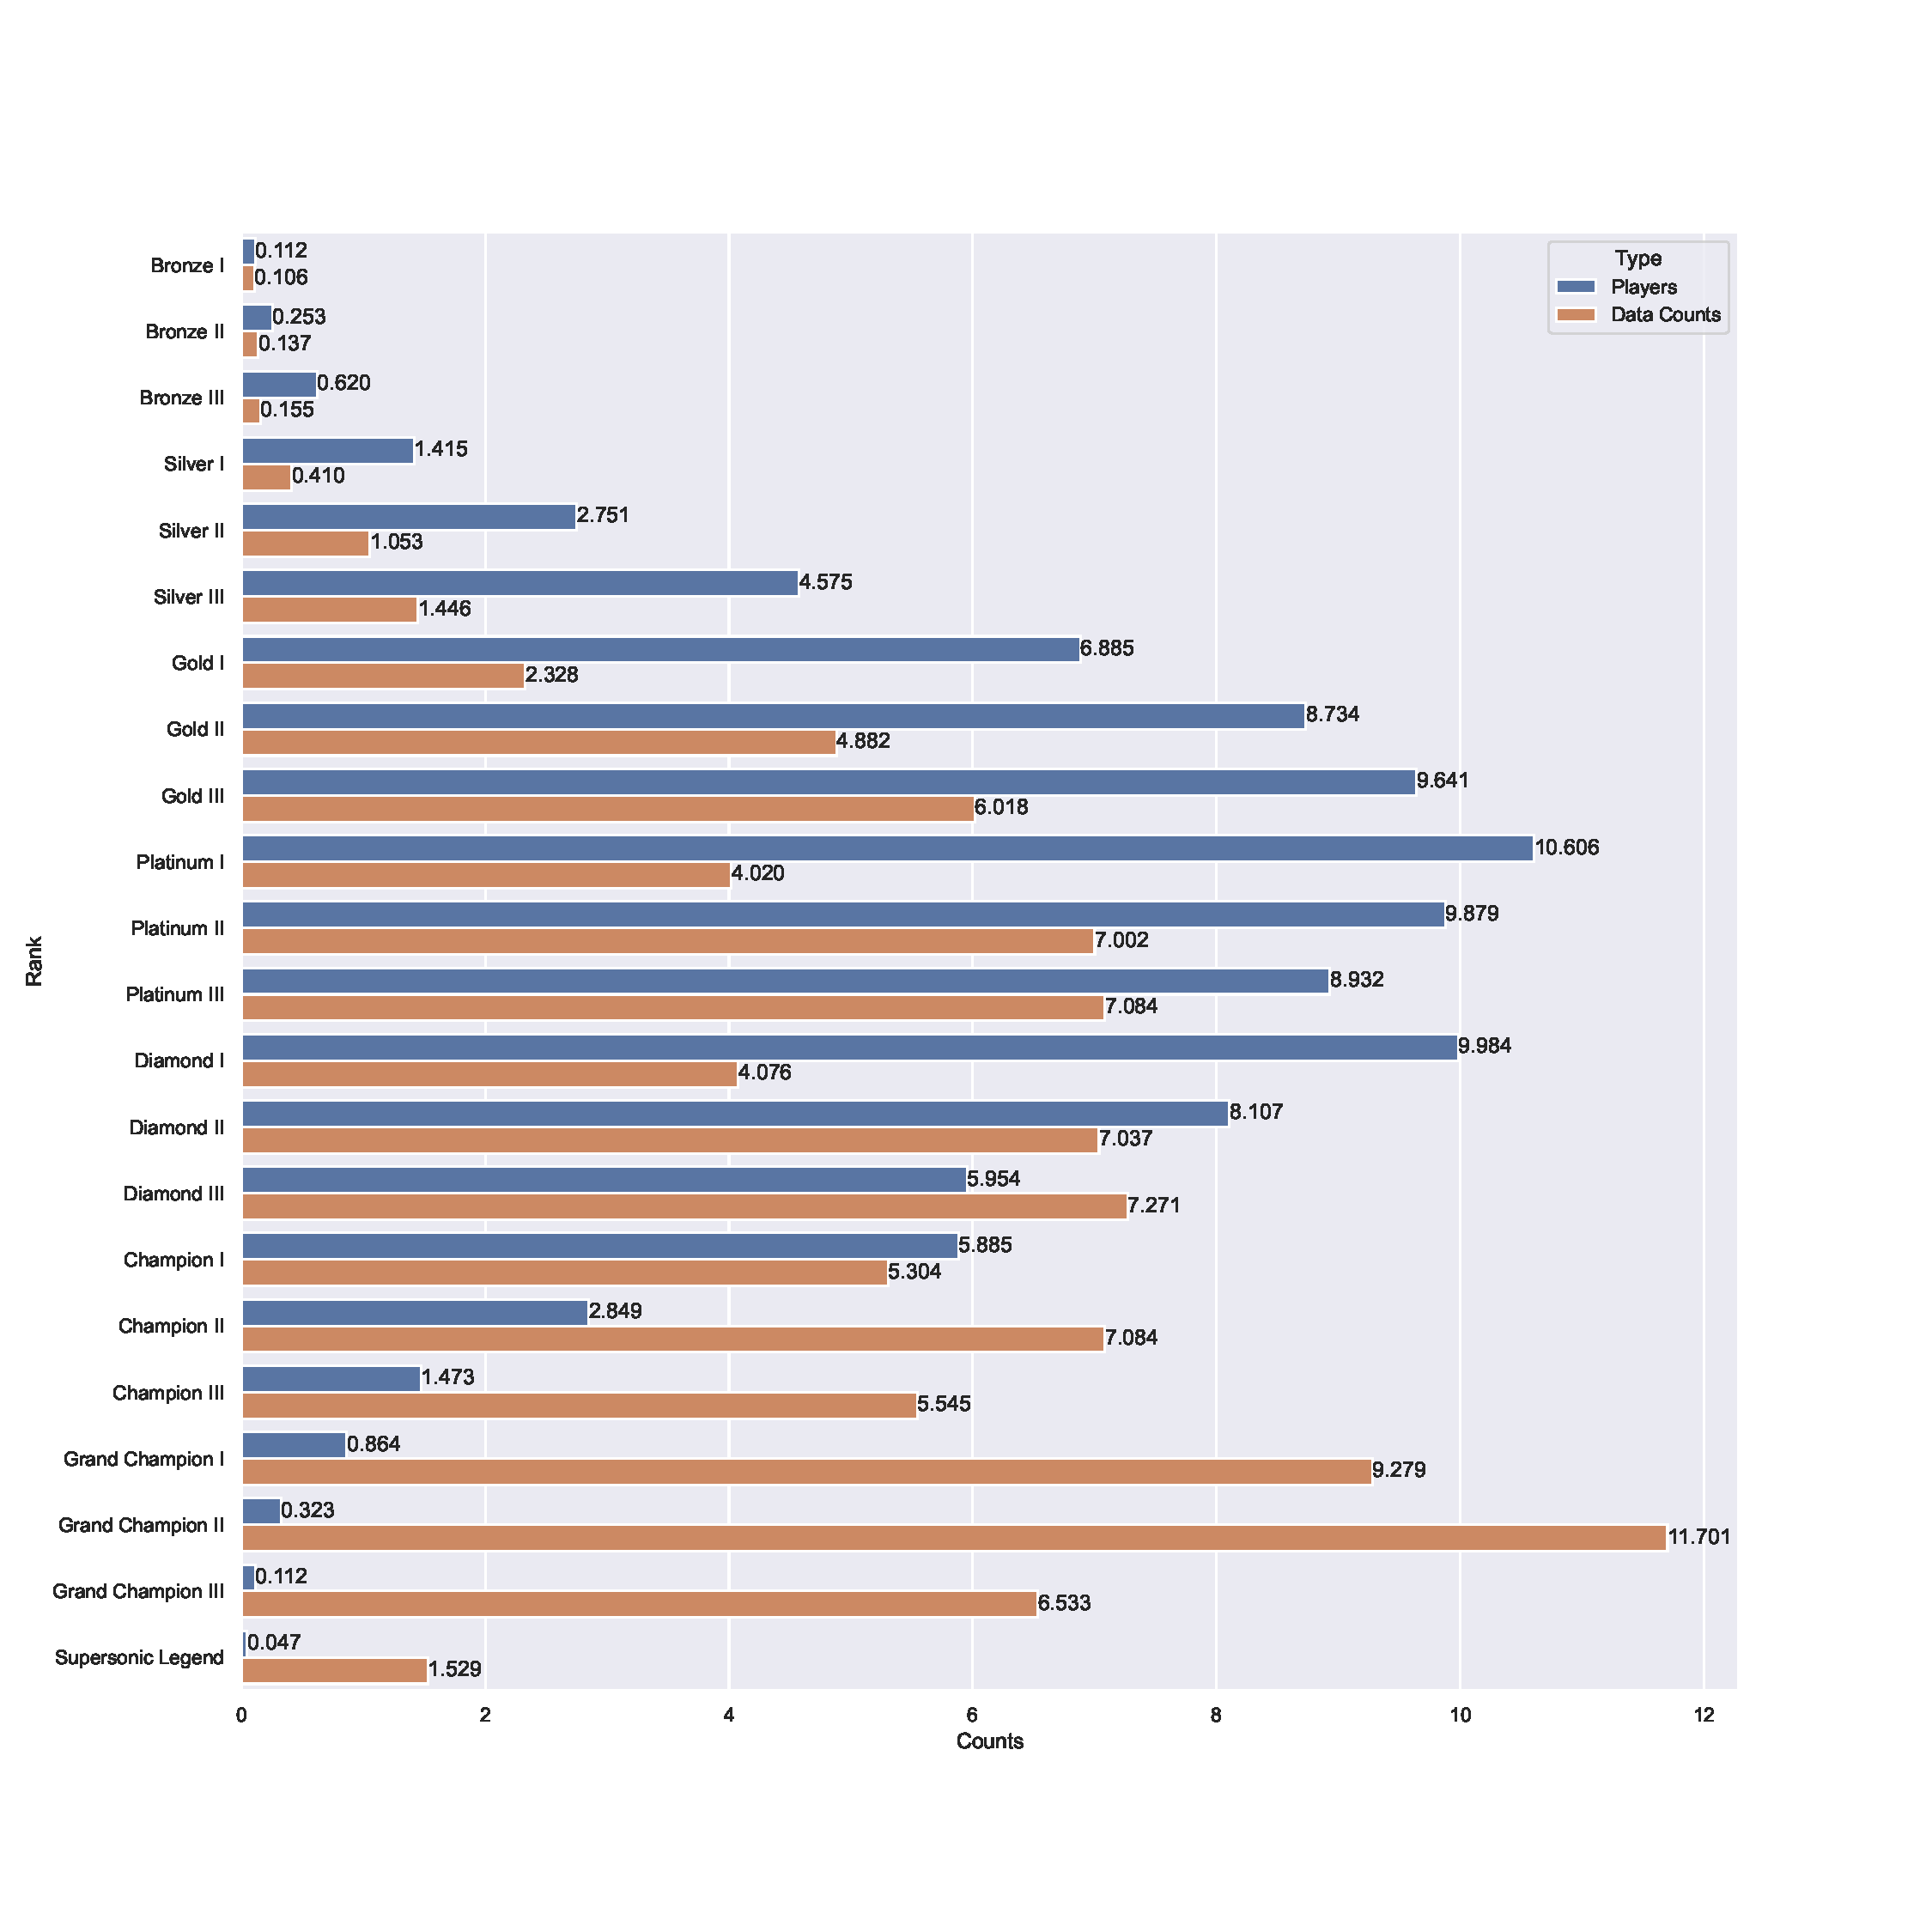
\includegraphics{res/imgs/tiers.pdf}}
    \label{fig:rank_distr}
    \caption{Distribution of players ranks (blue) vs. distribution of ranks in data (orange)}
\end{figure}

We can notice that the the bronze class had very few examples. This has two main reasons, the first one is that there are actually very few players in bronze, it's very difficult to get there basing on how ranking system works. The second reason is that players in bronze are casuals players that even don't know about the plugin necessary to upload replays. We can see the distribution of ranks for the current season (Season 5) in \reffig{fig:rank_distr} (orange). In the same figure we can see in blue the actual distribution of players, that is more or less normally distributed and centered. The data distribution is instead shifted to the right; as we said, skilled players tends to use and know about the plugin.

\subsubsection{Describe features}
We have 85 features in our data, let's briefly describe them

\begin{center}
    \textit{Core Stats}
\end{center}
\begin{itemize}
    \item \textbf{shots}: shots performed;
    \item \textbf{shot}\_against: shots the players undergoes while he is acting as goalkeeper;
    \item \textbf{goals}: goals performed,
    \item \textbf{goals\_against}: goals taken: 
    \item \textbf{saves}: goals saved,
    \item \textbf{assists}: assists performed,
    \item \textbf{score}: score cumulated at the end of the match,
    \item \textbf{mvp}: tells if is the most valuable player in the match,
    \item \textbf{shooting\_percentage}: shots compared to the teams shots
\end{itemize}
\begin{center}
    \textit{Boost Stats}
\end{center}
\begin{itemize}
    \item \textbf{bpm}: boost consumption per minute;
    \item \textbf{bcpm}: boost collected per minute;
    \item \textbf{amount\_collected\_big}: Amount of boost collected with big pads. Boost can be collected through big or mini pads, big ones are at the edges of the playing field, and fulls the boost, mini ones are scattered trough the field and refill only $13 \%$;
    \item \textbf{amount\_collected\_small}: amount of boost collected with mini pads;
    \item \textbf{amount\_stolen\_big}: amount of boost stolen to other players from big pads
    \item \textbf{amount\_stolen\_small}: amount of boost stolen to other players from mini pads
    \item \textbf{count\_collected\_big}: number of big pads taken,
    \item \textbf{count\_collected\_small}: number of mini pads taken,
    \item \textbf{amount\_overfill}: amount of boost extra boost taken from big pads
    \item \textbf{amount\_overfill\_stolen"}: amount of boost extra boost taken from big pads to steal from other players
    \item \textbf{amount\_used\_while\_supersonic"}: amount of boost used while in supersonic speed (useless as it is max speed)
    \item \textbf{time\_zero\_boost}: amount of time player has zero boost in the match;
    \item \textbf{time\_boost\_0\_25}: amount of time player has boost between 0 and 25;
    \item \textbf{time\_boost\_25\_50}: amount of time player has boost between 25 and 50;
    \item \textbf{time\_boost\_50\_75}: amount of time player has boost between 50 and 75;
    \item \textbf{time\_full\_boost}: amount of time player has full boost;
    \item \textbf{percent\_zero\_boost}: percent of time player has zero boost in the match;
    \item \textbf{percent\_boost\_0\_25}: percent of time player has boost between 0 and 25;
    \item \textbf{percent\_boost\_25\_50}: percent of time player has boost between 25 and 50;
    \item \textbf{percent\_boost\_50\_75}: percent of time player has boost between 50 and 75;
    \item \textbf{percent\_full\_boost}: amount of time player has full boost;
    \item \textbf{avg\_amount}: average amount of boost in the match;
\end{itemize}
\begin{center}
    \textit{Movement Stats}
\end{center}
\begin{itemize}
    \item \textbf{avg\_speed};
    \item \textbf{avg\_speed\_percentage}: average speed compare to max speed;
    \item \textbf{total\_distance}: total distance covered in the match
    \item \textbf{time\_slow\_speed}:  time spent moving slower than if you were boosting/dodging, i.e. just using throttle, less than ~1400 uu/s;
    \item \textbf{time\_boost\_speed}: time spent moving at boost speed, e.g. while holding boost/dodging, $~1400+ uu/s$; \\
    \item \textbf{time\_supersonic\_speed}: time spent moving at supersonic speed, $~ 2200+ uu/s$; \\
    \item \textbf{percent\_slow\_speed}: percentage time spent moving slower than if you were boosting/dodging, i.e. just using throttle, less than ~1400 uu/s;
    \item \textbf{percent\_boost\_speed}: percentage of time spent moving at boost speed, e.g. while holding boost/dodging, $~1400+ uu/s$; \\
    \item \textbf{percent\_supersonic\_speed}: percentage of time spent moving at supersonic speed, $~ 2200+ uu/s$; \\
    \item \textbf{time\_ground}: amount of time spent on the ground
    \item \textbf{time\_low\_air}: amount of time spent in air but at low altitude w.r.t. the field
    \item \textbf{time\_high\_air}: amount of time spent in air but at high altitude w.r.t. the field
    \item \textbf{percent\_ground}: percentage of time spent on the ground
    \item \textbf{percent\_low\_air}: percentage of time spent in air but at low altitude w.r.t. the field
    \item \textbf{percent\_high\_air}: percentage of time spent in air but at high altitude w.r.t. the field
    \item \textbf{time\_powerslide}: amount of time spent powersliding
    \item \textbf{count\_powerslide}: number of times player uses powerslide;
    \item \textbf{avg\_powerslide\_duration};
\end{itemize}
\begin{center}
    \textit{Positioning Stats}
\end{center}
\begin{itemize}
    \item \textbf{avg\_distance\_to\_ball};
    \item \textbf{avg\_distance\_to\_ball\_possession}: Average distance to the ball while possessing the ball
    \item \textbf{avg\_distance\_to\_ball\_no\_possession}: Average distance to the ball while not possessing the ball
    \item \textbf{avg\_distance\_to\_mates};
    \item \textbf{time\_defensive\_third}: amount of time player is in 1/3 of the field where his net is;
    \item \textbf{time\_neutral\_third}: amount of time player is in the neutral third;
    \item \textbf{time\_offensive\_third}: amount of time player is in 1/3 of the field where the opponent net is;
    \item \textbf{percent\_defensive\_third}: percentage of time player is in 1/3 of the field where his net is;
    \item \textbf{percent\_neutral\_third}: percentage of time player is in the neutral third;
    \item \textbf{percent\_offensive\_third}: percentage of time player is in 1/3 of the field where the opponent net is;
    \item \textbf{time\_offensive\_half}: amount of time player is in opponent half; \\
    \item \textbf{time\_defensive\_half}: amount of time player is in his team half; \\
    \item \textbf{percent\_offensive\_half}: percentage of time player is in opponent half; \\
    \item \textbf{percent\_defensive\_half}: percentage of time player is in his team half; \\
    \item \textbf{time\_behind\_ball}: amount of time the player is closer to its net than the ball; \\
    \item \textbf{time\_infront\_ball}: amount of time the player is closer to the opponent net than the ball; \\
    \item \textbf{percent\_behind\_ball}: percentage of time the player is closer to its net than the ball; \\
    \item \textbf{percent\_infront\_ball}: percentage of time the player is closer to the opponent net than the ball; \\
    \item \textbf{time\_farthest\_from\_ball}: amount of time he is the player farthest from ball; \\
    \item \textbf{time\_closest\_from\_ball}: amount of time he is the player closest from ball; \\
    \item \textbf{percent\_farthest\_from\_ball}: percentage of time he is the player farthest from ball; \\
    \item \textbf{percent\_closest\_from\_ball}: percentage of time he is the player closest from ball; \\
    \item \textbf{time\_most\_back}: amount of time he was the last defender of its team; \\
    \item \textbf{time\_most\_forward}: amount of time he was the first attacker of its team; \\
    \item \textbf{percentage\_most\_back}: amount of time he was the last defender of its team; \\
    \item \textbf{percentage\_most\_forward}: amount of time he was the first attacker of its team; \\
    \item \textbf{goals\_against\_while\_last\_defender};
\end{itemize}
\begin{center}
    \textit{Demolitions Stats}
\end{center}
\begin{itemize}
    \item \textbf{inflicted}: demolitions inflicted to opponent players;
    \item \textbf{taken}: demolitions taken by opponent players.
\end{itemize}

We can right away notice that there are a lot of features correlated, all the time / percent features are a repetition and we could keep only one among the twos.